\section{Acquisition Registration}
\label{section:acquisition-registration}

During an acquisition, multiple acquisitions are done and to each one corresponds a transformation (position and orientation) to the scene referencial. In this section, a method is described to find each one of this transformations, so all the acquisitions are merged into a single point cloud. The method chosen is the Iterative Closest Point, or ICP. This method is capable of aligning two point clouds, the reference and the target point cloud, by finding the transformation between the second to the first one. This is also known as point cloud registration.

\subsection{Iterative Closest Point}

\newcommand{\T}{\mathcal{T}}
\newcommand{\Pt}{\mathcal{P}}
\newcommand{\Q}{\mathcal{Q}}

This method can formally be described as follows: let $\Pt$ be the target point cloud and $\Q$ the reference point cloud. Then, the aim of the registration is to estimate the transformation $\T$ from the referencial of $\Pt$ to $\Q$ by minimizing the error function $\textrm{error}(\Pt, \Q)$ in \cref{eqn:icp-transformation-function}, where $\T(\Pt)$ is the result of the application of the transformation $\T$ to the point cloud $\Pt$.

\begin{equation}
\label{eqn:icp-transformation-function}
    \mathcal{T} = \underset{\T}{\textrm{argmin}}(\mathrm{error}(\T(\Pt), \Q))
\end{equation}

The error function $error(P, Q)$ is computed on pair of points that are associated between the two point clouds. This association is, ideally, between points that are closest in position in both point clouds. Then, the distance between the matching points $(p_i, q_i)$ are used in the error function in \cref{eqn:icp-error-function}. The matching algorithm can be based on features or geometric properties, so a better matching can be found. In this work, a simple point-to-point matching was used. 

\begin{equation}
\label{eqn:icp-error-function}
    \textrm{error}(\Pt, \Q) = \sum_{(p_i, q_i)}{|p_i - q_i|}
\end{equation}

In order to make the error function more robust, outlier points can be removed first from the match list. In addition, weights $w_i$ can be associated to each matching points $(p_i, q_i)$ to increase or decrease the influence of each matching points in the error function. As an example, normals can be used as a weight, so points with similar normals ($w_i = n_{p_i} \cdot n_{q_i}$) have a greater influence in the error function. 

However, the result of this minimization is always dependant on the association between the points, which, unless the descriptors are good enough (like visual correspondences), the matching is not perfect, and is worst the farther apart both point clouds are. The idea behind the ICP algorithm is that, even with a bag association, the resulting estimate can be used to find a better one. So, the ICP algorithm creates a series of transformation $\T_i$ at each iteration, yielding a new transformed point cloud $\Pt_i$. Then, the next transformation is found:

\begin{equation}
    \T_{i+1} = \underset{T}{\textrm{argmin}}(\textrm{error}(\T_i(\Pt_i), \Q))
\end{equation}

Finally, the final transformation estimate is the composition of all the intermediary transformations:

\begin{equation}
    \T = \T_1 \circ \T_2 \circ \dots \circ \T_N
\end{equation}

\subsection{Multiple Point Cloud ICP}
\label{section:multiple-pointcloud-icp}

ICP can only register pairs of point clouds, whereas this work requires a registration of $N$ point clouds, corresponding to $n$ acquisitions. So, a technique has to be found so that the ICP algorithm can be used with $n$ point clouds. Three of this such techniques are now describes, ordered by their complexity.

The first approach and the easier one to implement is to register each point clouds sequencially. In other words, this method registers the point cloud $\Pt_i$ to the point cloud $\Pt_{i-1}$ and the transformation $\T_{i-1}^{i}$ is found. The final accumulated point cloud is assembled using the \cref{eqn:registration-simple-method-calculation}. This method is the one that requires less overall registration, but has the disadvantage that the transformation errors increases for each successive point cloud. This approach is shown in \cref{figure:multiple-icp-method-1}.

\begin{equation}
\label{eqn:registration-simple-method-calculation}
    \Pt = \bigcup{\left(\T_1^2 \circ \T_2^3 \circ \dots \circ \T_{i-1}^i\right)(\Pt_i)}
\end{equation}

The next approach is widely used in robotics for Simultaneous Location and Mapping , or SLAM. This method holds an accumulated point cloud $A$ in memory, and each new incoming point cloud $\Pt$ registers to the accumulated point cloud.  Afterwards it is merged into $A$, which is then used for the next iteration, as shown in \cref{figure:multiple-icp-method-2}. It has the advantage that each new registration is done against a wider point cloud and has a smaller influence than in the previous method. Also, at each iteration the current pose of the 3D scanner is obtained, which is used as an initial estimate for the next iteration. However, the accumulated point cloud grows at each iteration, so a down-sampling is done at each iteration to keep the number of points bounded. In conclusion, each iteration can be calculated by \cref{eqn:icp-compose-1,eqn:icp-compose-2}.

\begin{align}
    \label{eqn:icp-compose-1}
    \T_{i} = & \textrm{ICP}(A, \Pt_{i}, \T_0 = \T_{i-1}) \\
    \label{eqn:icp-compose-2}
    A_{i+1} = & A{i} \bigcup \T_{i}(\Pt_i)
\end{align}

The last approach is the most complex. The idea of this approach is to minimize the number of transformation combinations, to minimize the propagation of the error. In particular, the registrations for the $N$ points clouds are done pairwise and are merged together to create $N/2$ point clouds. Then, this process is done recursively until an unique point cloud is obtained. This way, the maximum number of transformation combinations are equal to the number of levels of the tree, which is $\log_2(N)$, instead of $N$ combinations in the first approach. This algorithm is formalized in \cref{eqn:registration-tree-method-1,eqn:registration-tree-method-2}, for a list of point clouds $S=\left\{P_1, P_2, \ \dots, \ P_n\right\}$. At each level $l$ a new list of point clouds $^{l}P$ and transformations $^{l}T$ are computed, as shown in \cref{figure:multiple-icp-method-3}.

\begin{align}
    ^{l}\T = & \left\{\textrm{ICP}(^{l-1}\Pt_1, ^{l-1}\Pt_2), \ \dots, \ \textrm{ICP}(^{l-1}\Pt_{n-1}, ^{l-1}\Pt_{n}) \right\}
        \label{eqn:registration-tree-method-1} \\
    ^{l}\Pt = & \left\{^{l-1}\Pt_1 \bigcup{^{l}\T_1(^{l-1}\Pt_2}), \ \dots, \ ^{l-1}\Pt_{n-1} \bigcup{^{l}\T_{n/2}(^{l-1}\Pt_n)}\right\}
        \label{eqn:registration-tree-method-2}
\end{align}

In conclusion, three methods are possible to extend the ICP algorithm to multiple point clouds, and the three methods were used in this work and compared. After all the registrations are performed, point cloud can be assembled from all the point clouds, to form a big point cloud of the final scene. There is, however, a limitation of all this methods, because all of them have the principle that every point cloud is close to the previous one, which can be false. In this work, this was ensured in the capture methodology. 

\begin{figure}
    \centering
    \begin{subfigure}[t]{0.3\textwidth}
        \centering
        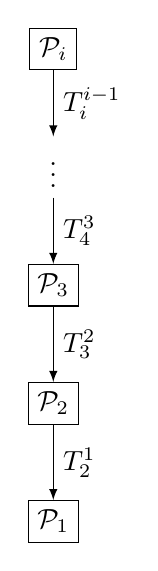
\begin{tikzpicture}
            \node[draw] (P1) at (0,0) {$\Pt_1$};
            \node[draw] (P2) at (0,1.5) {$\Pt_2$};
            \node[draw] (P3) at (0,3) {$\Pt_3$};
            \node (P4) at (0,4.5) {$\vdots$};
            \node[draw] (Pi) at (0,6) {$\Pt_i$};

            \draw[-latex] (P2) -- (P1) node[midway, anchor=west] {$T_2^1$};
            \draw[-latex] (P3) -- (P2) node[midway, anchor=west] {$T_3^2$};
            \draw[-latex] (P4) -- (P3) node[midway, anchor=west] {$T_4^3$};
            \draw[-latex] (Pi) -- (P4) node[midway, anchor=west] {$T_i^{i-1}$};
        \end{tikzpicture}

        \caption{First method}
        \label{figure:multiple-icp-method-1}
    \end{subfigure}%
    \begin{subfigure}[t]{0.3\textwidth}
        
        \centering
        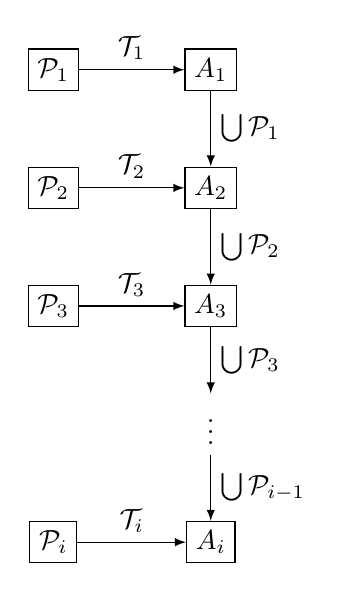
\begin{tikzpicture}
            \node[draw] (A1) at (0,0) {$A_1$};
            \node[draw] (A2) at (0,-1.5) {$A_2$};
            \node[draw] (A3) at (0,-3) {$A_3$};
            \node (A4) at (0,-4.5) {$\vdots$};
            \node[draw] (Ai) at (0,-6) {$A_i$};

            \node[draw, left of=A1, xshift=-1cm] (P1) {$\Pt_1$};
            \draw[-latex] (P1) -- (A1) node[midway, above] {$\T_1$};

            \node[draw, left of=A2, xshift=-1cm] (P2) {$\Pt_2$};
            \draw[-latex] (P2) -- (A2) node[midway, above] {$\T_2$};

            \node[draw, left of=A3, xshift=-1cm] (P3) {$\Pt_3$};
            \draw[-latex] (P3) -- (A3) node[midway, above] {$\T_3$};

            \node[draw, left of=Ai, xshift=-1cm] (Pi) {$\Pt_i$};
            \draw[-latex] (Pi) -- (Ai) node[midway, above] {$\T_i$};

            \draw[-latex] (A1) -- (A2) node[midway, right] {$\bigcup{\Pt_1}$};
            \draw[-latex] (A2) -- (A3) node[midway, right] {$\bigcup{\Pt_2}$};
            \draw[-latex] (A3) -- (A4) node[midway, right] {$\bigcup{\Pt_3}$};
            \draw[-latex] (A4) -- (Ai) node[midway, right] {$\bigcup{\Pt_{i-1}}$};
        \end{tikzpicture}

        \caption{Second method}
        \label{figure:multiple-icp-method-2}
    \end{subfigure}%
    \begin{subfigure}[t]{0.4\textwidth}
        
        \centering
        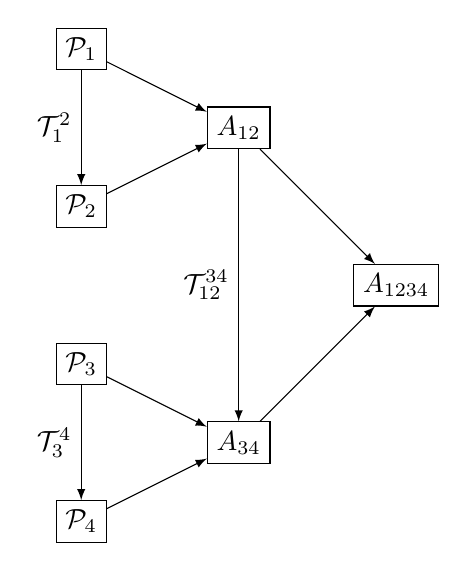
\begin{tikzpicture}
            \node[draw] (P1) at (0,0)  {$\Pt_1$};
            \node[draw] (P2) at (0,-2) {$\Pt_2$};
            \node[draw] (P3) at (0,-4) {$\Pt_3$};
            \node[draw] (P4) at (0,-6) {$\Pt_4$};

            \node[draw] (A12) at (2, -1) {$A_{12}$};
            \node[draw] (A34) at (2, -5) {$A_{34}$};
            \node[draw] (A1234) at (4, -3) {$A_{1234}$};

            \draw[-latex] (P1) -- (A12);
            \draw[-latex] (P2) -- (A12);
            \draw[-latex] (P3) -- (A34);
            \draw[-latex] (P4) -- (A34);
            \draw[-latex] (A12) -- (A1234);
            \draw[-latex] (A34) -- (A1234);

            \draw[-latex] (P1) -- (P2) node[midway, left] {$\T_1^2$};
            \draw[-latex] (P3) -- (P4) node[midway, left] {$\T_3^4$};
            \draw[-latex] (A12) -- (A34) node[midway, left] {$\T_{12}^{34}$};

        \end{tikzpicture}
        \caption{Third method}
        \label{figure:multiple-icp-method-3}
    \end{subfigure}%


    \caption{Multiple Point Cloud ICP approaches}
    \label{figure:registration-methods-approaches}
\end{figure}